% ------------------------------------------------------------------------
% ------------------------------------------------------------------------
% ------------------------------------------------------------------------
%                                Capítulo 3
% ------------------------------------------------------------------------
% ------------------------------------------------------------------------
% ------------------------------------------------------------------------

\chapter{METODOLOGÍA PROPUESTA}

El enfoque de red neuronal profunda propuesto para la clasificación de objetos desde medidas cuadráticas codificadas incluye tres etapas principales: (i) capa de adquisición, (ii) enfoque de inicialización, (iii) y red de clasificación. La Figura \ref{fig:esquema_entrenamiento} ilustra el esquema de red neuronal profunda propuesto. Primero, una capa de adquisición simula el proceso de medición \eqref{eq:phase_retrieval_problem}, donde la capa realiza un modelo de propagación del campo óptico. Luego, un procedimiento de inicialización aproxima el campo óptico $\mathbf{x}$, finalmente, la red de clasificación infiere la clase correspondiente a cada medida cuadrática codificada.


\begin{figure*}[!h]
    \centering
    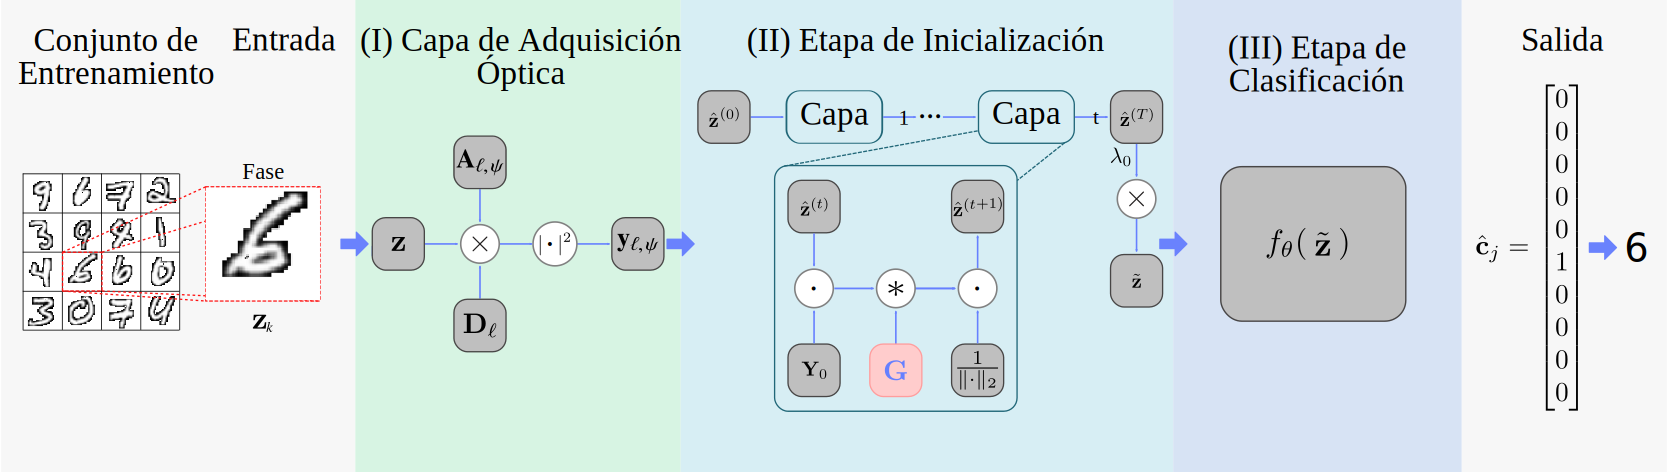
\includegraphics[width=\linewidth]{images/esquema_entrenamiento.pdf}
    \caption{Esquema de red neuronal profunda de tres etapas propuesto para la clasificación de objetos desde medidas cuadráticas codificadas.}
    \label{fig:esquema_entrenamiento}
\end{figure*}


\section{BLOQUE DE INICIALIZACIÓN}

Para realizar la etapa de inicialización del campo óptico, este trabajo toma ventaja del hecho de que la matriz de adquisición $\mathbf{A}_{\ell, \psi}$ es conocida, por lo tanto, se crea un mapeo $\mathcal{B}(\cdot)$ que pasa de las medidas $\mathbf{y}_{\ell, \psi}$ a una aproximación más cercana del campo óptico $\mathbf{x}$, dada por el desenvolvimiento de un algoritmo tradicional y un conjunto de capas convolucionales, de tal forma que $\hat{\mathbf{x}}=\mathcal{B}(\mathbf{A}_{\ell, \psi}, \mathbf{y}_{\ell, \psi})$. 

% El primer enfoque usa el operador de propagación hacia atrás inverso $\mathcal{P}_\ell:\mathbb{C}^n\rightarrow \mathbb{C}^n$ del campo óptico para aproximar$\hat{\mathbf{x}}$  \myfootcite{katkovnik2017computational}, que viene dado por

% \begin{equation}
%     \hat{\mathbf{x}}= \frac{1}{L}\sum_{\ell=1}^{ L} \mathcal{P}_\ell(\mathbf{y}_\ell).
%     \label{eq:back_propagation}
% \end{equation}

En concreto, este enfoque aplica un desenvolvimiento del algoritmo de inicialización de filtrado espectral (FSI\myfootcite{jerez2020fast}, por sus siglas en inglés). Esta inicialización se basa en un método de iteración de potencia para aproximar el campo óptico desde patrones codificados de difracción, el cual se resume en el Algoritmo \ref{alg_1}.

\begin{algoritmo}[!h]
    %\scriptsize
    \caption{Inicialización Espectral Filtrada}%\label{fsi_algo}
    \textbf{Entrada:} Matriz de sensado y medidas adquiridas $\{(\mathbf{A}_{\ell, \psi};\mathbf{y}_{\ell, \psi})\}_{\ell=1}^L$, máximo número de iteraciones $T$ y el filtro pasa bajas $ \mathbf{G}$.\newline
    \textbf{Salida:} $\hat{\mathbf{x}}$.
    \begin{algorithmic}[1]
        \State{$\tilde{\mathbf{x}}^{(0)} \leftarrow$ Aleatoriamente escogido}
        \State{ $ {\nu_\Xi}_\ell \left( \left( \mathbf{y}_{\ell, \psi} \right)_{i} \right) = 
                \begin{cases}
                1 & i \in \Xi_\ell \\
                0 & \text{De otra forma } \\
                \end{cases},1\leq i\leq n $
                }
        \State{ $ \tilde{\mathbf{y}}_{\ell, \psi} = \left[ {\nu_\Xi}_\ell \left( \left( \mathbf{y}_{\ell, \psi} \right)_1 \right),\cdots,{\nu_\Xi}_\ell \left( \left( \mathbf{y}_{\ell, \psi} \right)_n \right) \right]^T$ \Comment{Truncamiento por umbral} }
        \For{$t = 0: T-1$ }
        \State{$\tilde{\mathbf{x}}^{(t+1)} \leftarrow \sum_{\ell=1}^{L}\mathcal{P}_{\ell, \psi}\left(  \tilde{\mathbf{y}}_{\ell, \psi} \odot \mathbf{A}_{\ell, \psi}  \tilde{\mathbf{x}}^{(t)} \right) $ }
        \State{$\tilde{\mathbf{x}}^{(t+1)} \leftarrow {\mathbf{G}} * \tilde{\mathbf{x}}^{(t)}$\Comment{Operador de convolución}}
        
       \State{$\tilde{\mathbf{x}}^{(t+1)} \leftarrow \frac{\tilde{\mathbf{x}}^{(t+1)}}{{\Vert \tilde{\mathbf{x}}^{(t+1)} \Vert}_2 }$	\Comment{Normalización}}
        \EndFor
        \State{$\hat{\mathbf{x}}^{(T)} =  \tilde{\mathbf{x}}^{(T)} \sqrt{\frac{\sum_{\ell=1}^{L} \Vert\mathbf{y}_{\ell, \psi} \Vert_{2}^2 }{nL} } $\Comment{Escalado}}
    \end{algorithmic}
    \label{alg_1}
\end{algoritmo}

El algoritmo FSI crea el conjunto de índices $\Xi_\ell$ correspondientes a los valores más grandes de $\{(\mathbf{y}_{\ell, \psi})_{i}/\vert \vert\mathbf{a}_{\ell, \psi,i}\vert \vert_2\}$, donde $\mathbf{a}_{\ell, \psi,i}\in\mathbb{C}^{n}$ representan las filas de $\mathbf{A}_{\ell, \psi}$. Adicionalmente, el algoritmo incluye un filtro $\mathbf{G}$, el cual fue implementado como una capa convolucional, de tal manera que cada iteración del algoritmo FSI se aplica un filtrado que promueve mejoría en la aproximación, por lo tanto una mejora en la clasificación. 


\section{BLOQUE DE CLASIFICACIÓN}

En este trabajo se propone un esquema de clasificación de medidas cuadráticas codificadas. Para realizar la tarea de clasificación se puede usar diferentes modelos de clasificación, en este caso, se hizo uso de tres arquitecturas de clasificación del estado del arte, MobilNetV2 \myfootcite{mobilnetv2}, InceptionV3 \myfootcite{inceptionv3}  y Xception \myfootcite{xception}. La Tabla \ref{tab:comp_class_models} resume una comparación en número de parámetros, cantidad de capas y profundidad de las arquitecturas usadas.

\begin{table}[!h]
\centering
\begin{tabular}{|c|c|c|}
\hline
\textbf{Modelo}      & \textbf{Número de parámetros} & \textbf{Número de capas} \\ \hline
MobileNetV2 & 3,538,984            & 53              \\ \hline
InceptionV3 & 23,851,784           & 48              \\ \hline
Xception    & 22,910,480           & 71              \\ \hline
\end{tabular}
\caption{Resumen de las arquitecturas de redes neuronales de clasificación utilizadas.}
\label{tab:comp_class_models}
\end{table}

Para entrenar los pesos $\theta$ de la red de clasificación $f_\theta(\cdot)$, se puede usar el siguiente problema de optimización

\begin{equation}
    \mathbf{\theta}^* \in  \argmin_{\mathbf{\theta}} \frac{1}{J}\sum_{j = 1}^{J} \mathcal{L}\left( c^{(j)}, f_{\mathbf{\theta}}\left(\mathcal{B}(\mathbf{y}_{\ell}^{(j)})\right)\right).
    \label{eq:dl_optimization}
\end{equation}

Este problema minimiza la función pérdida usualmente llamada entropía categórica cruzada $\mathcal{L}(\cdot, \cdot)$ entre las etiquetas del dataset $c^{(j)}$, y las clases predichas $\hat{c}^{(j)} = f_\theta(\mathcal{B}(\mathbf{y}_{\ell, \psi}^{(j)}))$, donde $J$ es el número total de medidas y $\mathbf{y}_{\ell, \psi}^{(j)}$ es la medida cuadrática codificada al  j-ésimo ejemplo.


\section{ESQUEMA PROPUESTO DE CLASIFICACIÓN PROPUESTO}

El Algoritmo \ref{alg:algoritmo_2} resume el proceso de entrenamiento del esquema mostrado en la Figura \ref{fig:esquema_entrenamiento},  Para entrenar el esquema propuesto. Inicialmente, en la línea 2, el filtro de inicialización es inicializado usando una distribución uniforme $\mathcal{U}(\mathbf{0},\mathbf{1})$. Luego, el modelo de propagación descrito por la ecuación \eqref{eq:phase_retrieval_problem} es simulado por la capa de adquisición en la línea 5. Posteriormente se realiza el proceso de inicialización el cual aproximará las medidas cuadráticas codificadas al campo óptico inicial en la línea 6. Para obtener una clasificación se hace uso de el bloque de clasificación en la línea 7. En las líneas 8-10, el optimizador Adam $\mathcal{A}_{dam}(\cdot)$ se implementa para minimizar esta función de pérdida sobre el filtro de la inicialización y los parámetros de la red neuronal de clasificación ponderados por $\beta_1$ y $\beta_2$, respectivamente . Finalmente, estos parámetros óptimos $\mathbf{G}$ y $\boldsymbol{\theta}$ se retornan en la línea 13.


\begin{algoritmo}[!h]

        \caption{Enfoque de clasificación de objetivos.}
            \label{alg:algoritmo_2}
        	\begin{algorithmic}[1]
            \State{\textbf{Entrada:} Conjunto de entrenamiento $\{\mathbf{x}^{(k)}\}_{k=1}^\mathcal{K}$ con $\mathcal{K}$ imágenes.}  
            \State{\textbf{Inicialización filtro:} {\small
            $\mathbf{G}\in \mathcal{U}(\mathbf{0},\mathbf{1})^{5 \times 5}$} }
            \For{época = 1:$\mathcal{E}$}\Comment{$\mathcal{E}$ épocas}
                \For{$k= 1$:$\mathcal{K}$}\Comment{$\mathcal{K}$ ejemplos}
                    \State{$\mathbf{y}_{\ell,\psi} = \vert \mathbf{A}_{\ell,\psi}\mathbf{x}^{(k)}\vert^2, \quad \ell\in\{1,\dots,L\}$}
                    \Comment{Médidas cuadráticas codificadas}
                    \State{$\tilde{\mathbf{z}}^{(k)} \leftarrow  { \mathcal{B}\left(\mathbf{A}_{\ell,\psi},\mathbf{y}_{\ell, \psi}\right)}$}\Comment{Bloque de inicialización \ref{alg_1}}
                    \State{$\mathbf{c}^{(k)} \leftarrow  f_{\boldsymbol{\theta}}\left(\tilde{\mathbf{z}}^{(k)}\right)$}\Comment{Bloque de clasificación}
                    \State{$\mathcal{L}_{\mathbf{G},\boldsymbol{\theta}}=\frac{1}{\mathcal{K}}\sum_{k=1}^{\mathcal{K}} \mathcal{L}\left( c^{(k)}, f_{\mathbf{\theta}}\left(\mathcal{B}\left(\mathbf{A}_{\ell,\psi},\mathbf{y}_{\ell, \psi}\right)^{(k)}\right)\right) $}    
               \Comment{Función de costo}     
                    \State{$\mathbf{G}\leftarrow\mathcal{A}_{dam}( \mathbf{G}, \beta_1 \nabla_{\mathbf{G}} \mathcal{L}_{\mathbf{G},\boldsymbol{\theta}}) $}    
                \Comment{Optimización sobre $\mathbf{G}$ }
                      \State{$\boldsymbol{\theta}\leftarrow\mathcal{A}_{dam}( \boldsymbol{\theta}, \beta_2 \nabla_{\boldsymbol{\theta}} \mathcal{L}_{\mathbf{G},\boldsymbol{\theta}}) $}    
                \Comment{Optimización sobre $\boldsymbol{\theta}$ }
                \EndFor
                \EndFor
		\State{\textbf{Salida: } Kernel óptimo $\mathbf{G}$ y parámetros de la red neuronal $\boldsymbol{\theta}$.}
	\end{algorithmic}
	%\label{alg:algoritmo_2}
\end{algoritmo}
